% ======================================================================
\section{Decision Diagrams for BPO}
\label{sec:dds_for_bpo}

This section introduces the DD encoding used for BPO cut generation. In the context of integer and combinatorial optimization, DDs are graphical structures that encode the solution set of an optimization problem as paths. In what follows, we present the standard DD terminology~\cite{bergman2016decision,castroCireBeck2022survey,vanHoeve2024intro}.


Consider a combinatorial problem with $n$ binary variables and feasible set $X_B\subseteq\{0,1\}^n$.
A binary DD $B=(N,A)$ is a layered directed acyclic graph that represents $X_B$ as follows. Its node set is partitioned into layers $N=(N_1,\ldots,N_{n+1})$, where $N_1=\{r\}$ and $N_{n+1}=\{t\}$ contain the root and terminal node, respectively. Each transition from layer $i$ to layer $i+1$ corresponds to choosing the value of the
$i$-th variable in the order given to the DD. Thus, an arc $a=(u,u')\in A$, with
$u\in N_i$ and $u'\in N_{i+1}$, is labeled by a value $\val(a)\in\{0,1\}$. Each node
has at most one outgoing arc with value $0$ and at most one with value $1$. Then, a root-terminal path $p=(a_1,\ldots,a_n)$ encodes the binary vector $\bx^p=(\val(a_1),\ldots,\val(a_n))\in\{0,1\}^n$. Let $\mathcal{P}$ denote the set of all root-terminal paths; then we say that the DD is \emph{exact} if $X_B=\{\bx^p:p\in\mathcal{P}\}$, that is, each root-terminal path has a one-to-one correspondence with the solutions in $X_B$. 

%A common approach to measuring the size of a DD is to use its width. Specifically, the width of layer $i \in \{1,\ldots,n\}$ is the number of nodes in such layer (i.e., $|N_i|$), and the width of $B$ is given by $\max_{i \in \{1,\ldots,n\}} |N_i|$.

\subsection{A compact DD encoding for BPO} \label{subsec:compact_DD_bpo}

We now introduce our compact DD representation of BPO. This DD encoding is based on a dynamic programming (DP) model for BPO that considers only vertex variables as state variables, with hyperedge variables represented implicitly in the states. The DP model leverages that $z_e$ for $e \in E$ is completely defined by the assignment of its corresponding nodes since $z_e = \prod_{v \in e} z_v$.

We start by introducing some useful notation for the DP model. Consider a hypergraph $G=(V,E)$ that represents a BPO instance and a given vertex order $\sigma=(v_1,\ldots,v_n)$, where $n = |V|$. For $i\in \{0,\ldots,n\}$, let $U_0=\emptyset$ and $U_i=\{v_1,\ldots,v_i\}$, be the set of the first $i$ vertex decisions based on $\sigma$.  Then, we define the set of \textit{active hyperedges} with respect to $U_i$ as
$\A_i=\{e\in E : e\cap U_i\neq\emptyset,\ e\nsubseteq U_i\}$, that is, the set of hyperedges that have some vertex in $U_i$, but not all of them. We say that a hyperedge $e\in E$ is \emph{compatible} with the current partial assignment over the vertices in $U_i$ if every assigned vertex of $e$ has value one. 

We define our DP model with $n$ stages (i.e., one per vertex) such that the state variable at stage $i \in \{1,\ldots,n\}$ corresponds to the vertex variable $z_{v_i}\in\{0,1\}$ following the $\sigma$ order. State $s_i$ at stage $i \in \{1,\ldots,n\}$ is a subset of active hyperedges $\A_i$ that are compatible with respect to the current partial assignment. Given $s_0=\emptyset$ as the initial state, the transition function $\phi_i(s_{i-1},z_{v_i})$ at stage $i \in \{1,\ldots,n\}$ is given by
%
\[
\phi_i(s_{i-1},z_{v_i})=
\left\{
e\in\A_i :
\bigl(e\notin\A_{i-1}\ \text{or}\ e\in s_{i-1}\bigr)
\text{ and }
\bigl(v_i\notin e\ \text{or}\ z_{v_i}=1\bigr)
\right\}.
\]
The first condition considers the previously active hyperedges and potentially newly active hyperedges at stage $i$, while the second condition updates compatibility after assigning $v_i$. Intuitively, this encoding keeps track of the $\bz_e$ variables that can take the value one in each state (i.e., a compatible hyperedge) and ignores them if we have already assigned all vertices associated with a specific hyperedge. Formally, let
$\Ll_i=\{e\in E : v_i\in e,\ e\subseteq U_i\}$ be the hyperedges whose last vertex in  $\sigma$ is $v_i$ for every $i \in \{1,\ldots,n\}$. For every arc that assigns $z_{v_i}$, a hyperedge $e \in \Ll_i$ has its value assigned: $z_e = 1$ if it is compatible before assigning $v_i$ and $z_{v_i}=1$; and $z_e = 0$ otherwise.

Given this DP model, the DD is built in a top-down fashion from the root (i.e., initial state $s_0$) by applying the transition function at each layer
and merging nodes with equal states. Exactness with respect to $\mathcal{S}_G$
follows because the state keeps the needed information to determine which unfinished hyperedges can still attain value $1$ under future assignments, and therefore to recover every vector $(\bz_v,\bz_e)$. See Example \ref{exa:bpo-dd} for an illustrative example.

\begin{example}\label{exa:bpo-dd}
Consider a BPO instance with vertices $\{v_1, v_2, v_3\}$ and hyperedges $e_1=\{v_1, v_2\}$ and $ e_2=\{v_2, v_3\}$ and its associated compact DD as depicted in Figure \ref{fig:example-dd}. Nodes depict the states, solid black arcs are $1$-arcs (i.e., $z_{v_i}=1$) and dashed gray arcs are $0$-arcs (i.e., $z_{v_i}=0$). Given order $\sigma=(v_1,v_2,v_3)$, we have $U_1 = \{v_1\}$, $U_2 = \{v_1, v_2\}$, $U_3 = \{v_1, v_2, v_3\}$ and active hyperedge sets $\A_1 = \{e_1\}$, $\A_2 = \{e_2\}$, and $\A_3 = \emptyset$. Note that the states of the DD indeed encode the set of hyperedges $e\in E$ that could have $z_e = 1$ but have not yet been assigned. For instance, after assigning $z_{v_1}$, we have a state where either $e_1$ still has options of being selected (i.e., when $z_{v_1} =1$) or not (i.e.,  when $z_{v_1} = 0$).
\end{example}

\begin{figure}
	\centering
    % Hypergraph (vertical layout) for V={v1,v2,v3}, E={e1={v1,v2}, e2={v2,v3}}.
% Vertices are nodes; hyperedges are solid enclosing regions overlapping on v2.
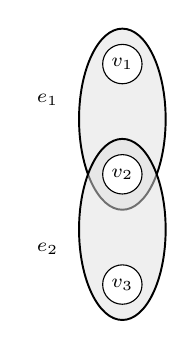
\begin{tikzpicture}[
    vertex/.style={circle, draw, fill=white, font=\scriptsize,
                   minimum size=0.5cm, inner sep=1pt},
    hedge/.style={draw, line width=0.7pt, fill=gray!25, fill opacity=0.5}
  ]

  % --- hyperedges (drawn first, behind the vertices) ---
  \draw[hedge] (0,-0.7) ellipse [x radius=0.55, y radius=1.15];
  \draw[hedge] (0,-2.1) ellipse [x radius=0.55, y radius=1.15];

  % --- hyperedge labels ---
  \node[font=\scriptsize] at (-0.95,-0.45) {$e_1$};
  \node[font=\scriptsize] at (-0.95,-2.35) {$e_2$};

  % --- vertices ---
  \node[vertex] (v1) at (0,  0  ) {$v_1$};
  \node[vertex] (v2) at (0, -1.4) {$v_2$};
  \node[vertex] (v3) at (0, -2.8) {$v_3$};

\end{tikzpicture}

    \hspace{5em}
	% Compact DD for the BPO instance V={v1,v2,v3}, E={e1={v1,v2}, e2={v2,v3}}.
% Style adapted from the bdd-lifting paper: dashed grey = 0-arcs, solid black = 1-arcs.
\begin{tikzpicture}[
    >=Stealth, thick,
    state node/.style={ellipse, draw, fill=gray!12, font=\scriptsize,
                       minimum width=1.05cm, minimum height=0.55cm, inner sep=1pt},
    zero arc/.style={draw, dashed, gray, ->, line width=0.5pt},
    one arc/.style={draw, ->, line width=0.6pt},
    layer label/.style={font=\scriptsize\itshape, gray}
  ]

  % --- nodes (state = active hyperedges still compatible) ---
  \node[state node] (r)  at ( 0,    0  ) {$\emptyset$};
  \node[state node] (u1) at (-1, -1) {$\emptyset$};
  \node[state node] (u2) at ( 1, -1) {$\{e_1\}$};
  \node[state node] (u3) at (-1, -2) {$\emptyset$};
  \node[state node] (u4) at ( 1, -2) {$\{e_2\}$};
  \node[state node] (t)  at ( 0,   -3) {$\emptyset$};

  % --- layer (variable) annotations on the left ---
  \node[layer label] at (-2,-0.5) {$v_1:$};
  \node[layer label] at (-2,-1.5) {$v_2:$};
  \node[layer label] at (-2,-2.5) {$v_3:$};

  % --- arcs ---
  \path
    (r)  edge[zero arc] (u1)
         edge[one arc]  (u2)
    (u1) edge[zero arc] (u3)
         edge[one arc]  (u4)
    (u2) edge[zero arc] (u3)
         edge[one arc]  (u4)
    (u3) edge[zero arc, bend right=18] (t)
         edge[one arc,  bend left=18]  (t)
    (u4) edge[zero arc, bend right=18] (t)
         edge[one arc,  bend left=18]  (t);

  % --- legend ---
  \node (l0a) at (2.3,-0.15) {};
  \node[anchor=west, font=\scriptsize] (l0b) at (2.7,-0.15) {$z_{v_i}=0$};
  \node (l1a) at (2.3,-0.65) {};
  \node[anchor=west, font=\scriptsize] (l1b) at (2.7,-0.65) {$z_{v_i}=1$};
  \path (l0a) edge[zero arc] (l0b.west)
        (l1a) edge[one arc]  (l1b.west);

\end{tikzpicture}

	\caption{BPO instance as a hypergraph (left) and its associated DD encoding (right).}
	\label{fig:example-dd}
\end{figure}


\subsection{An extended formulation induced by the compact DD}
\label{subsec:compact_DD_extended_formulation}

A simple way to use an exact DD inside an LP formulation is through its network-flow representation \cite{behle2007}. This formulation assumes that every variable of the problem is explicitly represented in the DD (i.e., it corresponds to one of the decisions in each layer).  In what follows, we adapt such a model to our compact DD encoding, in which hyperedge variables are implicitly represented. 

Let $B=(N,A)$ be the compact DD associated with $G=(V,E)$ and  assume vertex order $\sigma=(v_1,\ldots,v_n)$. For an arc $a\in A$, let $s(a)$ and $t(a)$ denote its source and target nodes, respectively, and consider sets $\Aout(u)=\{a\in A:s(a)=u\}$ and $\Ain(u)=\{a\in A:t(a)=u\}$ to represent outgoing and incoming arcs of a node $u \in N$. Lastly, if $a \in A$ leaves layer $N_i$, then $\var(a)=v_i$ is the vertex associated with arc $a$ and $\val(a)\in\{0,1\}$ is its assigned value.

We now define the arcs that assign each variable $(\bz_v, \bz_e)$ to the value one or zero. For a vertex $v\in V$, let $\Gamma_v^1=\{a\in A:\var(a)=v,\ \val(a)=1\}$ and $\Gamma_v^0=\{a\in A:\var(a)=v,\ \val(a)=0\}$ be the set of arcs associated with the $z_v = 1$ and $z_v = 0$ decisions, respectively. For hyperedge variables, recall that $\Ll_i$ is the set of hyperedges whose value can be deduced when $v_i$ is assigned, for each $i \in \{1,\ldots,n\}$. For each arc $a \in \Aout(u)$ leaving a node $u \in N_{i}$ with state $s_{i-1}$, we define
$
\E_1(a)=
\{e\in\Ll_i:e\in s_{i-1},\ \val(a)=1\}$,
and 
$\E_0(a)=\Ll_i\setminus\E_1(a)
$
as the sets of hyperedges assigned value 1 and 0 on arc $a$, respectively. Lastly, for each $e\in E$, $\Gamma_e^1=\{a\in A:e\in\E_1(a)\}$ and $\Gamma_e^0=\{a\in A:e\in\E_0(a)\}$ are the set of arcs that define the $z_e$ variable to 1 and 0, respectively. 

To create the extended formulation for BPO based on the DD $B=(N,A)$, consider $y_a\geq0$ a continuous flow variable associated with arc $a\in A$. Then, the network flow model associated with $B$ is:
%
\begin{subequations}\label{model:bpo-extended-dd}
\begin{align}
    \min\ & \sum_{v\in V} c_v z_v + \sum_{e\in E} c_e z_e \label{eq:flow-objective} \\
   \st\ & \sum_{a\in \Aout(u)} y_a - \sum_{a\in \Ain(u)} y_a = 0 & \forall u\in N\setminus\{r,t\}, \label{eq:flow-all}\\
   & \sum_{a\in \Aout(r)} y_a = \sum_{a\in \Ain(t)} y_a = 1, \label{eq:flow-root-terminal}\\
   & z_j = \sum_{a\in\Gamma_j^1} y_a & \forall j \in V\cup E, \label{eq:flow-link}\\
   & y_a \geq 0 & \forall a \in A. \label{eq:flow-vars}
\end{align}
\end{subequations}

Constraints \eqref{eq:flow-all} and \eqref{eq:flow-root-terminal} are the standard network-flow constraints over a DD, whose feasible flows are exactly the convex combinations of root-terminal paths; thus, they encode $\conv(X_B)$. Constraints \eqref{eq:flow-link} link the flow to the BPO variables: $z_v$ accumulates the flow on the arcs that set $z_v=1$, and $z_e$ accumulates the flow on the arcs where the compact DD implicitly finalizes $z_e=1$. Since every root-terminal path crosses exactly one arc of $\Gamma_j^1\cup\Gamma_j^0$ for each $j\in V\cup E$, these identities are well defined, and the objective \eqref{eq:flow-objective} coincides with the BPO objective \eqref{eq:bpo-objective}. The validity of the model and the fact that the projection of \eqref{eq:flow-all}--\eqref{eq:flow-vars} onto the $(\bz_v,\bz_e)$ variables equals $MP_G$ follow directly from the compact DD encoding and Theorem 4.1 of~\cite{behle2007}.
